\documentclass[12pt]{article} \usepackage{url, graphicx}

% page layout
\setlength{\topmargin}{-0.25in}
\setlength{\textheight}{9.5in}
\setlength{\headheight}{0in}
\setlength{\headsep}{0in}

% problem formatting
\newcommand{\problemname}{Problem}
\newcounter{problem}

% math
\newcommand{\dd}{\mathrm{d}}

% primary units
\newcommand{\rad}{\mathrm{rad}}
\newcommand{\kg}{\mathrm{kg}}
\newcommand{\m}{\mathrm{m}}
\newcommand{\s}{\mathrm{s}}

% secondary units
\renewcommand{\deg}{\mathrm{deg}}
\newcommand{\km}{\mathrm{km}}
\newcommand{\mi}{\mathrm{mi}}
\newcommand{\h}{\mathrm{h}}
\newcommand{\ns}{\mathrm{ns}}
\newcommand{\J}{\mathrm{J}}
\newcommand{\eV}{\mathrm{eV}}
\newcommand{\W}{\mathrm{W}}

% derived units
\newcommand{\mps}{\m\,\s^{-1}}
\newcommand{\mph}{\mi\,\h^{-1}}
\newcommand{\mpss}{\m\,\s^{-2}}

% random stuff
\sloppy\sloppypar\raggedbottom\frenchspacing\thispagestyle{empty}

\begin{document}

\noindent
Name: \rule[-1ex]{0.55\textwidth}{0.1pt}
NetID: \rule[-1ex]{0.2\textwidth}{0.1pt}

\section*{NYU Physics I---Final Exam}

\paragraph{\problemname~\theproblem:}\refstepcounter{problem}%
Assume that Professor Hogg has a mass of exactly $70\,\kg$. Now
consider a very realistic, stone statue of Professor Hogg that is
twice his size in every direction (twice as tall, and realistic). What
would be the mass of this statue, approximately?
(From Lecture, 2018-09-06.)

\vfill

\paragraph{\problemname~\theproblem:}\refstepcounter{problem}%
Roughly what is terminal velocity for a 1-liter soda bottle, filled
with soda (or pop or juice or whatever), falling from a tall building?
(From Problem Set 1.)

\vfill

\paragraph{\problemname~\theproblem:}\refstepcounter{problem}%
We spent time talking about two vectors, $\vec{v}_3$ and $\vec{v}_4$,
which were the velocities of the rock on a no-air-resistance trajectory.
What was wrong with this picture, that we drew?
\marginpar{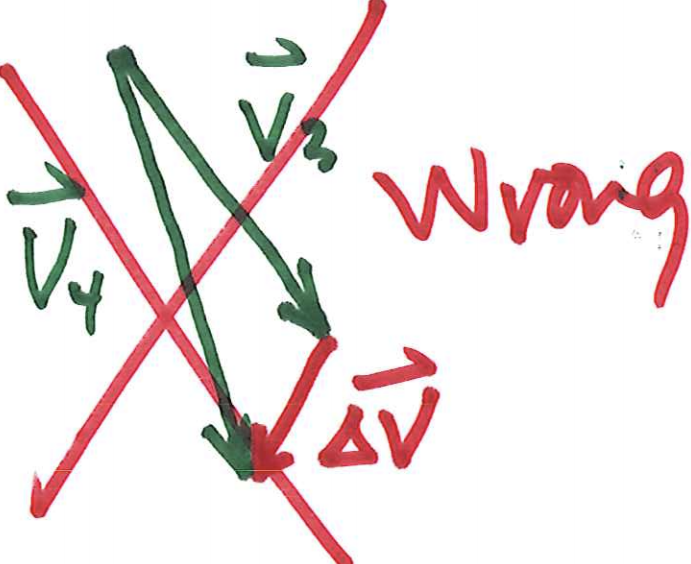
\includegraphics[width=1in]{../jpg/wrong_vectors.png}}
(From Term Exam 1.)

\vfill
~
\clearpage

\paragraph{\problemname~\theproblem:}\refstepcounter{problem}%
Consider a $1\,\kg$ stone thrown upwards at an initial upward velocity of
magnitude $10\,\mps$. Plot the vertical velocity (with upwards
positive) as a function of time for the first 2 seconds of its
trajectory. Use a gravitational acceleration of $10\,\mpss$. Label
your axes quantitatively. Ignore air resistance.
(From Problem Set 2.)

\vfill

\paragraph{\problemname~\theproblem:}\refstepcounter{problem}%
What is the magnitude $|\vec{N}|$ of the normal force acting on a package of
mass $M$ sitting on the floor of an elevator that is accelerating
upwards with acceleration magnitude $a$. The elevator is an ordinary
elevator in an ordinary building in New York City.
(From Problem Set 3.)

\vfill

\paragraph{\problemname~\theproblem:}\refstepcounter{problem}%
A car is going around a banked turn faster than the speed for which
the bank is designed. Therefore the car is relying on lateral friction
to make the turn!  Draw a free-body diagram for the car, showing at
least the gravitational force, the normal force, and the frictional
force.
(From Problem Set 4.)

\vfill
~
\clearpage

\paragraph{\problemname~\theproblem:}\refstepcounter{problem}%
You have a block of mass $m$ on an inclined plane, inclined at an
angle $\theta=15\,\deg$ to the horizontal. The coefficient of friction
is $\mu=0.9$. What is the magnitude of the frictional force on the
block? The acceleration due to gravity is $g$.
You must leave your answer in terms of $\mu$, $m$, $g$, $\theta$, or
whatever you need to deliver a correct symbolic answer.
Once again, state any assumptions you need to make.
(From Term Exam 2.)

\vfill

\paragraph{\problemname~\theproblem:}\refstepcounter{problem}%
A roller coaster zooms over the top of a hill of radius $4\,\m$ (such that the
center-of-mass of the car and people are moving on a circular trajectory of
radius $4\,\m$). At what speed $v$ should the roller coaster go if the people in
the car are going to nearly feel weightless? Use $g=10\,\mpss$, and give
a numerical answer in $\mps$.
(From Lecture 2018-09-27.)

\vfill

\paragraph{\problemname~\theproblem:}\refstepcounter{problem}%
A package of mass $m$ is moving at a horizontal velocity of magnitude $v$ at $t=0$
relative to the floor.  It scrapes to a halt on the floor. How much
heat $Q$ is generated by the friction, from $t=0$ until when the
package comes to rest?
(From Problem Set 5.)

\vfill
~
\clearpage

\paragraph{\problemname~\theproblem:}\refstepcounter{problem}%
A $0.16\,\,kg$ ball is dropped from a height of $1\,\m$ onto a concrete
floor. If the bounce takes only $10^{-4}\,\s$, what was the (approximate)
magnitude of the force on the ball from the floor? Give a numerical
answer in $\N$.
(From Lecture 2018-10-11.)

\vfill

\paragraph{\problemname~\theproblem:}\refstepcounter{problem}%
Without using a calculator, estimate the sine of the angle $1.2~\deg$.
Use the small-angle approximation! (\emph{Hint:} Degrees aren't radians.)
(From Term Exam 3.)

\vfill

\paragraph{\problemname~\theproblem:}\refstepcounter{problem}%
If I stretch a spring, I am experiencing Hooke's law. What is the
stress and what is the strain in this case? Answer in words!
(From Lecture 2018-10-18.)

\vfill
~
\clearpage

\paragraph{\problemname~\theproblem:}\refstepcounter{problem}%
A typical adult is holding her or his left arm at a right angle, so
the upper arm is pointing straight down, and the forearm is pointing
horizontally forwards. The hand is oriented palm-up. The arm is
holding a 6 kg grocery bag by its handle in the hand. Draw a diagram
showing the forces acting on the forearm+hand system, at roughly the locations
where they are acting. You can think of it as being the forces on the forearm+hand
bones if that makes more sense.
(From Problem Set 7.)

\vfill

\paragraph{\problemname~\theproblem:}\refstepcounter{problem}%
If you have a potential of the form
$$
U(x) = A\,x^3 - B\,x + C
$$ where $A$ and $B$ and $C$ are positive constants, find a location ($x$ position) at which
the force is zero.
(From Term Exam 4.)

\vfill

\paragraph{\problemname~\theproblem:}\refstepcounter{problem}%
If I tell you that the position $x$ of a particle is moving with
time according to the equation:
\begin{equation}
x(t) = B\,\e^{-\frac{\Gamma}{2}\,t}\,\cos (2\pi\,f\,t + \theta)
\quad ,
\end{equation}
then what are the units of $B$, $\Gamma$, $f$ and $\theta$?
(From Problem Set 8.)

\vfill
~
\clearpage

\paragraph{\problemname~\theproblem:}\refstepcounter{problem}%
A bungy cord has a natural (unstretched) length of $5\,\m$ and it
stretches by $1\,\m$ for every $400\,\N$ of applied force. How much
energy is the bungy cord storing when it is stretched to
a total length of $7\,\m$? Give a numerical answer in $\J$.
(From Problem Set 9.)

\vfill

\paragraph{\problemname~\theproblem:}\refstepcounter{problem}%
How is it that the astronauts in the Space Station are weightless?
Write a grammatically correct answer in one sentence, in fewer than 17
words.  Box your sentence!
(From Term Exam 5.)

\vfill

\paragraph{\problemname~\theproblem:}\refstepcounter{problem}%
A car of mass $M$ is accelerating at acceleration $a$ in the $x$
direction. Its center of mass is a height $h$ above the ground.  What
is the net torque on the car, if any, when you consider the reference point to be
a point that is stationary and \emph{on the ground}?
(From Problem Set 10.)

\vfill
~
\clearpage

\paragraph{\problemname~\theproblem:}\refstepcounter{problem}%
What is escape velocity from the surface of the Earth? That is, how
fast do you have to move to get out of Earth's gravity?
If you don't remember $G$ or $M$ for the Earth (and you shouldn't remember
those!) then remember that $g = G\,M/R^2$ and the radius $R$ of the Earth is
about $6300\,\km$.
Give a numerical answer in $\mps$.
(From Problem Set 11.)

\vfill

\paragraph{\problemname~\theproblem:}\refstepcounter{problem}%
If the Earth were four times less massive than it is, but were still
on a circular orbit at its current orbital radius (semi-major axis),
how much longer or shorter would the year be?  (From Worksheet on
orbits.)

\vfill

\paragraph{\problemname~\theproblem:}\refstepcounter{problem}%
Sketch an orbit of roughly eccentricity 0.9. Most importantly: Show the
point about which the object is orbiting, and make sure your pericenter
and apocenter distances make sense. Don't worry about getting it all right,
just roughly!
(From Term Exam 6.)

\vfill
~
\clearpage

\paragraph{\problemname~\theproblem:}\refstepcounter{problem}%
What, roughly, is $\gamma$ for the astronauts in the Space Station,
according to a scientist stationary in the Earth rest frame?
(From Problem Set 13.)

\vfill

\paragraph{\problemname~\theproblem:}\refstepcounter{problem}%
A particle of mass $M$ is at rest. It decays into two identical
photons traveling in the positive and negative $x$ directions.
What are the 4-momenta of these two photons?
(From Problem Set 14.)

\vfill

\paragraph{\problemname~\theproblem:}\refstepcounter{problem}%
Two balls of putty of mass $m$ are fired towards each other in outer space.
They collide and stick perfectly, without losing any putty or
radiating any sound or heat or anything else. Is the combined blob
of putty created by this collision slightly more than, slightly less
than, or exactly equal to $2\,m$ in mass? And say why, in fewer than
17 words. Make your answer correct to at least first order in
$\beta^2$. That is, the weakly relativistic limit. But I only need
a qualitative answer, don't calculate anything! (From Lecture
2018-12-13.)

\vfill
~
\end{document}
